\chapter{Methodology}
\label{cha:methodology}

This chapter details the methodology employed to integrate ControlNet into the MESA model for steerable terrain generation. The process encompasses problem definition, dataset construction, preprocessing, terrain feature extraction, model architecture design, training strategy, loss function formulation, validation, logging procedures, and implementation specifics.

\section{Problem Definition}
\label{sec:problem_definition}

The primary objective of this thesis is to enhance the controllability of diffusion-based terrain generation by integrating the ControlNet architecture into the MESA model. The task involves training a model to generate realistic heightmaps conditioned on specific terrain features extracted from digital elevation models. The inputs to the model include Sentinel-2 satellite imagery, DEM tiles, cloud masks, text prompts, and algorithmically extracted terrain feature maps. The model is trained to produce heightmaps that not only align with the provided text prompts but also adhere to the spatial structure defined by the terrain feature maps.

\section{Dataset Construction}
\label{sec:dataset_construction}

MajorTOM~\cite{schulz2024majortom} is used as the primary data source for training. It provides paired Sentinel-2 satellite imagery and digital elevation models across a wide range of geographic locations and conditions. The dataset also includes cloud masks that identify occluded regions. Text prompts are taken from the MESA~\cite{borne-pons2025mesa} base model metadata. The dataset is filtered to remove invalid and low-quality samples.

\subsection{Data Sources}
\label{subsec:data_sources}

The training data consists of the MajorTOM~\cite{schulz2024majortom} Core-DEM and Core-S2L2A datasets. The Core-DEM dataset provides digital elevation models at 10\,m resolution, while the Core-S2L2A dataset contains Sentinel-2 Level 2A imagery and cloud masks. The text prompts are derived from the model metadata, which includes text prompts for each grid cell. For filtering, the Global 100\,m Terrestrial Human Footprint dataset~\cite{gassert2023hfp100} is used to exclude areas with significant human impact.

\subsection{Filtering and Selection}
\label{subsec:filtering_and_selection}

The dataset is filtered to ensure that only valid and informative samples are included in training. DEM tiles with over 20\% of missing data are excluded, as are samples with a Human Footprint~(HFP) score of over 10. These values were chosen to balance the need for a large training set with the desire to focus on natural terrain features.

\subsection{Dataset Format}
\label{subsec:dataset_format}

The final dataset is stored in a parquet format with columns for the Sentinel-2 color bands, DEM tiles, cloud masks, text prompts, and any additional metadata. During training, these columns are accessed and processed in the preprocessing pipeline to prepare the inputs for the model.

\section{Preprocessing Pipeline}
\label{sec:preprocessing_pipeline}

The preprocessing pipeline takes raw bytes from the dataset and converts them into tensors suitable for model input. Sentinel-2 imagery is decoded from the RGB bands, resized to 768$\times$768 via linear interpolation, and normalized to the [-1,~1] range. DEM tiles are decoded and normalized by dividing by the local, per-tile maximum elevation to ensure values are in a consistent range. They are then resized to 768$\times$768 and rescaled to the [-1,~1] range. Cloud masks are decoded and resized to 768$\times$768 via nearest-neighbor interpolation, resulting in binary tensors where 1 indicates cloud cover and 0 indicates clear sky.

\section{Terrain Feature Map Generation}
\label{sec:terrain_feature_map_generation}

In order to provide spatial conditioning that captures meaningful terrain structure, feature maps consisting of ridges, valleys, and cliffs are extracted from the DEMs. Following Lochner et al.~\cite{lochner2023interactive}, flow accumulation is used to identify valleys, while the flow accumulation of the inverted DEM is analyzed to find ridges. Cliffs are detected using Canny edge detection combined with slope thresholds. This process is shown in Figure~\ref{fig:feature_map_extraction}. After extracting these features, dropout is applied based on the Strahler number to randomly drop parts of the control signal during training, which encourages the model to learn from partial conditioning and improves robustness. The Strahler number is used to bias the dropout towards main ridge- and valley lines, which are more important for the overall terrain structure. The resulting feature maps are combined into a three-channel tensor, with each channel representing one of the terrain features. This combined feature map is then used as conditioning input for the ControlNet branch of the model.


\begin{figure}[htbp]
	\centering
	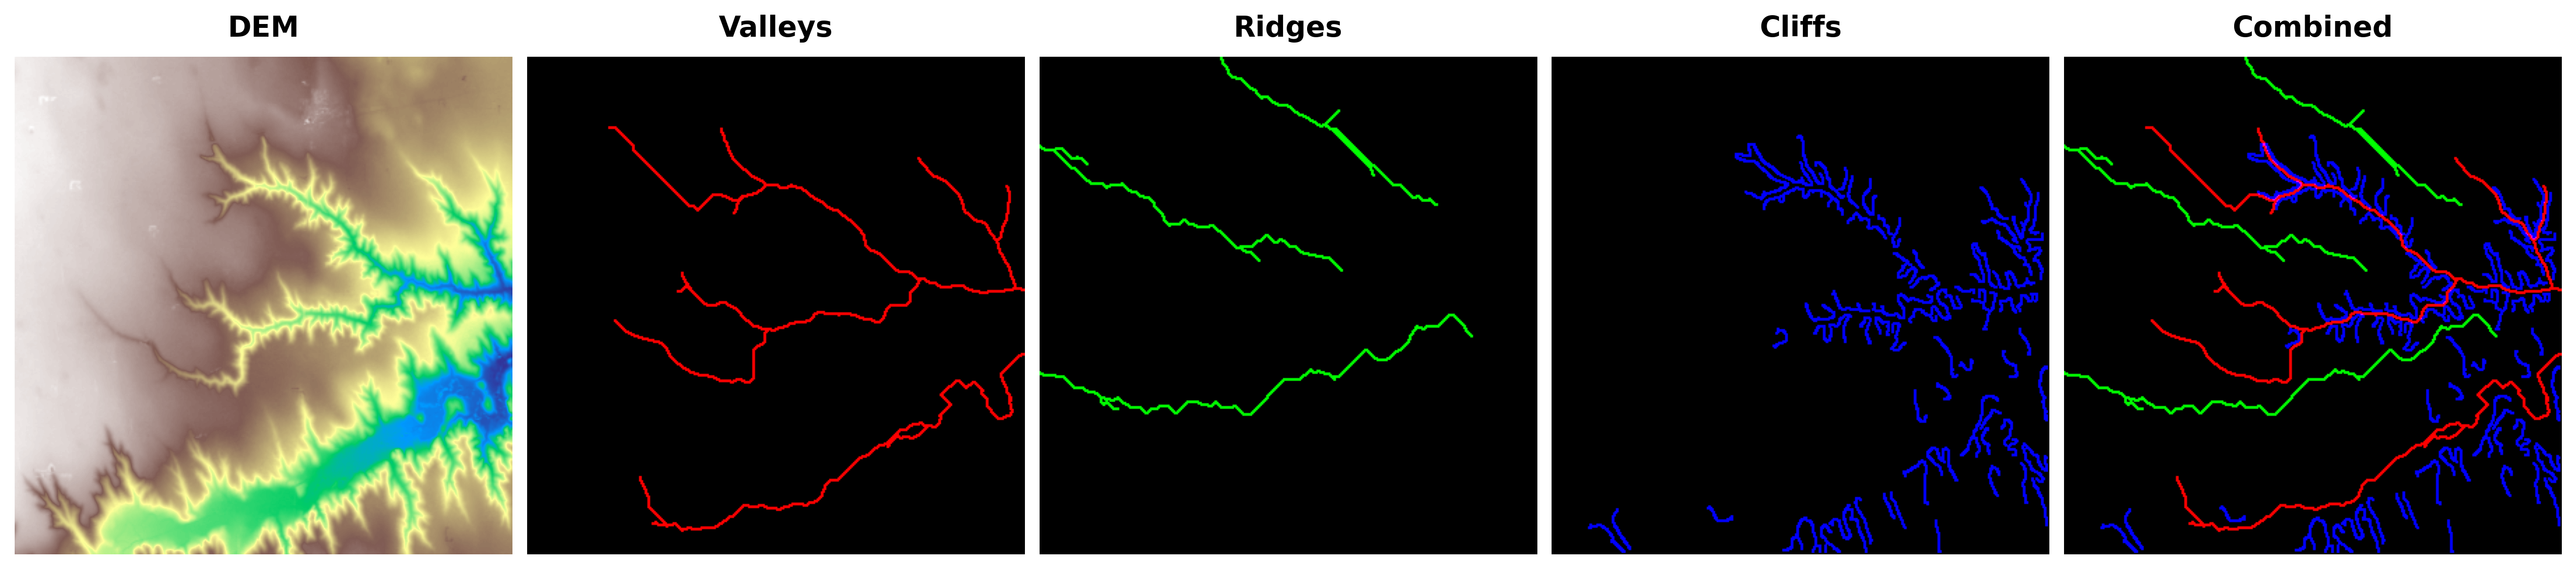
\includegraphics[width=\linewidth]{images/feature_map_extraction.png}
	\caption{Side-by-side comparison of an original DEM and the extracted terrain feature maps. From left to right: the input DEM rendered with a terrain color map, valleys (red channel), ridges (green channel), cliffs (blue channel), and the combined three-channel feature map.}
	\label{fig:feature_map_extraction}
\end{figure}

\pagebreak[0]

\section{Model Architecture}
\label{sec:model_architecture}

For the ControlNet model, the down blocks of the MESA~\cite{borne-pons2025mesa} U-Net are duplicated to create a separate conditioning branch. The ControlNet branch receives the noisy latent sample with the conditioning feature maps added. To keep training stable, the conditioning feature map is passed through a zero-initialized convolution. The conditioned samples are then passed through the cloned down blocks. The resulting residuals from the ControlNet are passed through a zero-initialized convolution and added to the main U-Net residuals at the corresponding layers. The rest of the U-Net architecture remains frozen, allowing the pretrained weights to be leveraged while still enabling spatial conditioning through the ControlNet branch.

\section{Training Strategy}
\label{sec:training_strategy}

The training loop samples random batches of data, applies the preprocessing pipeline, and feeds the inputs through the model to compute the loss. The VAE, text encoder, and base U-Net are frozen during training, while only the ControlNet parameters are updated. For classifier-free guidance, a random subset of prompts is replaced with empty strings during training.

\subsection{Noise Scheduling and Timesteps}
\label{subsec:noise_scheduling_and_timesteps}

The training loop samples random diffusion timesteps for each batch, and noise is added to the input samples according to the noise scheduler. The model is trained to predict either the noise or velocity, depending on the configuration. This approach allows the model to learn to denoise across a range of noise levels, improving its ability to generate high-quality samples during inference.

\subsection{Optimization and Efficiency}
\label{subsec:optimization_and_efficiency}

For optimization, AdamW, 8-bit AdamW, or Prodigy optimizers are evaluated, with Prodigy ultimately chosen. Gradient accumulation is employed to achieve an effective batch size larger than what fits in memory. Mixed precision training is used to reduce memory usage and speed up training. Gradient checkpointing is also utilized to further reduce memory consumption. Additionally, \texttt{torch.compile} and attention backend choices are explored to optimize performance.

\section{Loss Function}
\label{sec:loss_function}

The primary loss function used during training is the mean squared error (MSE) between the predicted noise or velocity and the target noise or velocity. This loss encourages the model to learn to denoise the input samples effectively across different noise levels. Additionally, weighting terms as detailed in Sections~\ref{subsec:snr_weighted_loss_method} and~\ref{subsec:cloud_masked_loss_weighting} are used to balance the contribution of different timesteps or regions.

\subsection{SNR-Weighted Loss}
\label{subsec:snr_weighted_loss_method}

SNR-weighted loss is applied to balance the learning across different noise levels. By weighting the loss according to the signal-to-noise ratio at each timestep, the model is encouraged to focus more on learning to denoise samples at noise levels where the signal is stronger, while still learning from noisier samples~\cite{hang2024efficientdiffusiontrainingminsnr}.

\subsection{Cloud-Masked Loss Weighting}
\label{subsec:cloud_masked_loss_weighting}

Following MESA~\cite{borne-pons2025mesa}, cloud masks are used to ignore the loss contribution from cloudy regions during training. This prevents the model from learning to create cloudy outputs. By focusing the loss on clear sky regions, the model can learn to generate unoccluded terrain features.

\section{Validation and Logging}
\label{sec:validation_and_logging}

Validation and logging are essential components of the training process to monitor progress and evaluate model performance. The following subsections detail the specific strategies used for validation sampling and training diagnostics.

\subsection{Validation Sampling}
\label{subsec:validation_sampling}

A fixed set of validation samples is selected from the training distribution for qualitative monitoring. These samples are used to generate outputs at regular intervals during training, allowing for qualitative inspection of the generated terrain features. Quantitative metrics such as mIoU between predicted and reference feature maps are also tracked to provide a more objective measure of performance.

\subsection{Training Diagnostics}
\label{subsec:training_diagnostics}

During training, various diagnostics are tracked to monitor the optimization process. This includes tracking the training loss, learning rate, gradient norms, and control signal norms. Any anomalies in these diagnostics can provide insights into potential issues with the training setup or model architecture.

\section{Implementation Details}
\label{sec:implementation_details}

The training is implemented using PyTorch 2.8.0, with Diffusers 0.35.2 for the diffusion model architecture. Accelerate 1.10.1 is used to manage distributed training and mixed precision. Transformers 4.57.1 is used for text tokenization and encoding. Geospatial libraries such as rasterio 1.4.3, pysheds 0.5, and richdem 0.3.4 are used for processing DEMs and extracting terrain features. Additional supporting libraries include torchvision 0.23.0, bitsandbytes 0.47.0, and ProdigyOpt 1.1.2. The software stack is designed to be compatible with both Linux and Windows platforms.
Training was done on a single NVIDIA RTX 3090 with 24\,GB of VRAM for 28 hours for the first training run~(16k steps), and 55 hours for the second training run~(40k steps).
